\ifx \globalmark \undefined %% This is default.
	\documentclass[twoside,openright,11pt,a4paper]{report}

%\compiler avec xelatex
%\usepackage[applemac]{inputenc}
\usepackage[T1]{fontenc}
\usepackage[utf8]{inputenc} %latin1 est possible
%\usepackage[latin1]{inputenc} %latin1 est possible
\usepackage[francais]{babel}
\usepackage{lettrine}

\usepackage[text={13cm,20cm},centering]{geometry}

\renewcommand{\familydefault}{cmss}

\usepackage{graphicx}
\usepackage{amsmath}
\usepackage{amsfonts}
\usepackage{amssymb}
\usepackage{amsthm}
\usepackage{bm}
\usepackage{color}

\newcommand{\real}{\mathbb{R}}
\newcommand{\mb}{\mathbf}
\newcommand{\bos}{\boldsymbol}

\def \RR {I \! \! R}

\newcommand{\e}{\begin{equation}}  
\newcommand{\ee}{\end{equation}}
\newcommand{\eqn}{\begin{eqnarray}} 
\newcommand{\eeqn}{\end{eqnarray}} 
\newcommand{\eqnn}{\begin{eqnarray*}} 
\newcommand{\eeqnn}{\end{eqnarray*}} 

\newcommand{\bpm}{\begin{pmatrix}}
\newcommand{\epm}{\end{pmatrix}}

%\newcommand{\{\c c}}{\c c}

\newcommand{\bma}{\left(\begin{array}}
\newcommand{\ema}{\end{array}\right)} 
\newcommand{\hh}{\hspace{2mm}}
\newcommand{\hd}{\hspace{5mm}}
\newcommand{\hu}{\hspace{1cm}}
\newcommand{\vv}{\vspace{2mm}}
\newcommand{\vd}{\vspace{5mm}}
\newcommand{\vm}{\vspace{-2mm}}
\newcommand{\teq}{\triangleq}
%\newcommand{\qedb}{\,$\Box$}
\newcommand{\blanc}{$\left. \right.$}
\newcommand{\frts}[2]%
         {\frac{{\textstyle #1}}{{\textstyle #2}}}

\newcommand{\bindex}[3]%
{
\renewcommand{\arraystretch}{0.5}
\begin{array}[t]{c}
#1\\
{\scriptstyle #2}\\
{\scriptstyle #3}
\end{array}
\renewcommand{\arraystretch}{1}
}

\theoremstyle{definition}
\newtheorem{exemple}{{\bf Example}}[chapter]
\newtheorem{theoreme}[exemple]{{\bf Theorem}}
\newtheorem{propriete}[exemple]{{\bf Property}}
\newtheorem{definition}[exemple]{{\bf Definition}}
\newtheorem{remarque}[exemple]{{\bf Remark}}
\newtheorem{remarques}[exemple]{{\bf Remarks}}
\newtheorem{lemme}[exemple]{{\bf Lemma}}
\newtheorem{hypothese}[exemple]{{\bf Hypothesis}}
\newtheorem{exercice}{{\bf Exercise}}[chapter]

\newcommand{\xqedhere}[2]{%
 \rlap{\hbox to#1{\hfil\llap{\ensuremath{#2}}}}}

\newcommand{\xqed}[1]{%
 \leavevmode\unskip\penalty9999 \hbox{}\nobreak\hfill
 \quad\hbox{\ensuremath{#1}}}

\newcommand{\gf}{\fg\,\,}

\newcommand{\cata}[1] %
     {\renewcommand{\arraystretch}{0.5}
     \begin{array}[t]{c} \longrightarrow \\ {#1} \end{array}
     \renewcommand{\arraystretch}{1}}

\usepackage[isu]{caption}
%\usepackage[font=small,format=plain,labelfont=bf,up,textfont=it,up]{caption}
\setlength{\captionmargin}{60pt}

\newcommand{\cqfd}
{%
\mbox{}%
\nolinebreak%
\hfill%
\rule{2mm}{2mm}%
\medbreak%
\par%
}

\pagestyle{headings}

\renewcommand{\sectionmark}[1]{%
\markright{\thesection.\ #1}{}}

\renewcommand{\chaptermark}[1]{%
\markboth{\chaptername\ \thechapter.\ #1}{}}

\makeatletter 
\def\@seccntformat#1{\csname the#1\endcsname.\;} 
\makeatother

\title{ {\Huge {\textbf{Modélisation et analyse  \\ \vspace{4mm} des systèmes dynamiques }}} \\ \vspace{4cm} G. Bastin}

%\title{ {\Huge {\textbf{Modelisation et analyse  \\ \vspace{4mm} des systemes dynamiques }}} \\ \vspace{4cm} G. Bastin}


\date{\today}
	\begin{document} %% Crashes if put after (one of the many mysteries of LaTeX?).
\else 
	\documentclass{standalone}
	\begin{document}
\fi

\graphicspath{ {Chapitre2/images/} }


\setcounter{chapter}{1}
\chapter{Systèmes mécaniques articulés}
\chaptermark{Systèmes mécaniques articulés}\label{systmeca}




\lettrine[lines=1]{\bf L}{}e sujet de ce chapitre est la mise en équation des modèles d'état des systèmes 
mécaniques formés d'un ensemble de corps rigides reliés entre eux par des articulations. La méthode systématique de modélisation que nous allons étudier s'applique à de nombreux exemples pratiques de systèmes mécaniques tels que les véhicules (automobiles, trains, avions,...) ou les robots. Cette méthode résulte d'une application systématique de la loi de Newton. 

Dans le but de simplifier les notations et les calculs nous nous li\-mi\-terons à 
l'établissement des équations du mouvement dans un espace à deux dimensions
(c'est à dire dans un plan). L'extension au cas d'un mouvement dans un
espace à trois dimensions est conceptuellement élémentaire mais plus difficile
à visualiser. 

Nous considérons 
tout d'abord le cas d'un corps rigide unique en l'absence de frottement. Ensuite, nous traitons la modélisation d'un système articulé constitué de plusieurs corps rigides. La méthode de modélisation est présentée en détail à l'aide d'un exemple de robot manipulateur à deux degrés de liberté. Enfin nous examinons comment étendre le modèle pour prendre en compte le frottement, l'élasticité des articulations et les contraintes non-holonomes.

\section{Dynamique d'un corps rigide dans le plan}

Nous considérons un corps rigide se déplaçant dans un plan dans lequel une
base inertielle orthonormale $0, X_b, Y_b$ est fixée arbitrairement 
(Fig.\ref{Fig:corigidplan}).
\begin{figure}[h]
\begin{center}
\includegraphics[width=6cm]{corigidplan}
\caption{Coordonnées d'un corps rigide dans le plan}
\label{Fig:corigidplan}
\end{center}
\end{figure}
Un vecteur $\vec{W}$ est attaché au corps. La position
du corps est complètement spécifiée par les 3 coordonnées $x, y, \theta$: 
\begin{itemize}
\item $x, y$ sont les coordonnées cartésiennes du centre de masse $G$ dans la base
fixe $0,X_b,Y_b$~;
\item $\theta$ est l'orientation du vecteur $\vec{W}$ par rapport à la base fixe $0,X_b,Y_b$. 
\end{itemize}
Nous définissons le vecteur de dimension 3 décrivant la position du corps :
\eqn
q \triangleq \bma{c} x \\y \\ \theta \ema. \label{cogen}
\eeqn

\noindent Une application directe des lois de Newton, coordonnée 
par coordonnée, conduit alors aux équations générales du mouvement suivantes :

\begin{itemize}
\item Equations de translation du centre de masse :
\eqnn
m\ddot{x} &=& F_x, \\ m\ddot{y} &=& F_y.
\eeqnn
\item Equation de rotation autour du centre de masse :
\eqnn
I\ddot{\theta} = T.
\eeqnn
\end{itemize}

\noindent où $m$ est la masse du corps, $I$ est son moment d'inertie par rapport au centre
de masse,
$F_x$ et 
$F_y$ désignent les projections de la résultante des forces appliquées au corps sur 
les axes $0X_b$ et $0Y_b$ 
respectivement, $T$ est la résultante des moments des forces appliquées
pour la rotation du corps autour du centre de masse.

Ces équations générales du mouvement constituent la base de l'éta\-blis\-sement 
du modèle d'état du système comme nous allons l'illustrer dans un exemple.

\begin{exemple}{\bf Modélisation de la dynamique d'une fusée.}

Nous considérons une fusée se déplaçant dans un plan perpendiculaire à
la terre. La fusée est propulsée par deux moteurs à réaction disposés symétriquement
par rapport au corps de la fusée comme indiqué sur la Figure \ref{Fig:fusee}. 
\begin{figure}[ht]
\begin{center}
\includegraphics[width=8cm]{fusee}\hfill
\includegraphics[width=4.6cm]{ariane}
\caption{Modélisation de la dynamique d'une fusée - Photo de la fusée Ariane au décollage (\copyright \,ESA)}
\label{Fig:fusee}
\end{center}
\end{figure}
Les équations du mouvement sont établies sous {\bf l'hypothèse de modélisation} que la fusée
constitue un corps rigide de masse constante. 
\begin{itemize}
\item Equations de translation :
\begin{equation} \begin{split} \label{transfus}
m\ddot{x} &= F_x = (F_1 + F_2)\cos\theta, \\ 
m\ddot{y} &= F_y = (F_1 + F_2)\sin\theta - mg_0.  
\end{split} \end{equation}
\item Equation de rotation :
\eqn
I\ddot{\theta} = T = (F_2 - F_1)d\sin\alpha. \label{rotfus}
\eeqn
\end{itemize}
\noindent 
Dans ces équations, $(x,y)$ est la position du centre de masse $G$, $\theta$ l'angle du vecteur $\vec W$ par rapport à l'horizontale, $F_{1}, F_{2}$ les poussées des réacteurs, $m$ la masse de la fusée, $I$ son moment d'inertie, $d, \alpha$ des paramètres géométriques (Fig.\ref{Fig:fusee}) et $g_0$ la constante de gravitation.

Les équations (\ref{transfus})-(\ref{rotfus}) se mettent sous la forme standard d'un modèle d'état $\dot{x} =
f(x,u)$ de dimension 6 avec deux entrées si l'on introduit les notations suivantes~:
\begin{description}
\item {\em Variables d'état:}
\eqnn
x_1 = x, \hspace{6mm} x_2 = y, \hspace{6mm} x_3 = \theta, \hspace{6mm} x_4 = \dot{x}, \hspace{6mm} 
x_5 = \dot{y}, \hspace{6mm} x_6 = \dot{\theta}.
\eeqnn
\item {\em Variables d'entrée :}
\eqnn
u_1 = F_1, \hspace{10mm} u_2 = F_2.
\eeqnn
\end{description}
Le modèle d'état s'écrit comme suit~:
\begin{equation*} \begin{split}
\dot x_1 &= x_4, \\
\dot x_2 &= x_5, \\
\dot x_3 &= x_6, \\
\dot x_4 &= \frac{\cos x_3}{m} (u_1 + u_2), \\
\dot x_5 &= - g_0 + \frac{\sin x_3}{m} (u_1 + u_2), \\
\dot x_6 &= \frac{d \sin \alpha }{I} (u_2 - u_1). \qed
\end{split} \end{equation*}
\end{exemple}

Une situation particulière appara\^it lorsque
le corps considéré est soumis à un ensemble de forces
dont la résultante est nulle mais qui ne sont pas toutes appliquées au même point. Les
équations du mouvement s'écrivent alors :
\eqnn
m\ddot{x} &=& 0\\ 
m\ddot{y} &=& 0 \\
I\ddot{\theta} &=& T 
\eeqnn
Dans un tel cas, il est d'usage dans certaines applications de ne pas spécifier les forces qui
sont à l'origine du moment $T$ mais de considérer directement celui ci comme la cause du
mouvement. On dit, pour simplifier, que le corps est soumis à un {\em couple}. C'est ainsi par
exemple que l'on parlera du couple fourni par un moteur pour faire tourner un segment de
robot manipulateur.

Le modèle d'état obtenu dans l'exemple de la fusée est non-linéaire par
rapport aux variables d'état et affine par rapport aux variables d'entrée. Ce sera le cas
pour la plupart des applications qui nous intéressent et pour lesquelles les équations de
translation  et de rotation décrivant la dynamique d'un corps rigide peuvent s'écrire sous
la forme matricielle générale :
\eqnn
J\ddot{q} + b(q) = B(q)u.
\eeqnn
Dans cette équation $J$ est la matrice (diagonale et constante) d'inertie, $b(q)$
représente l'effet de la gravitation et 
$B(q)$ est une
matrice (dite cinémati\-que) dépendant non-linéairement des variables d'état. 
On en déduit que le
modèle d'état s'écrit sous la forme générale suivante :
\eqnn
\dot{q} &=& v, \\ 
\dot{v} &=& J^{-1}[-b(q) + B(q)u],
\eeqnn
où $v \triangleq \dot{q}$ est appelé {\em vecteur des vitesses généralisées}.

\section{Dynamique des systèmes mécaniques articulés}

Nous considérons maintenant le cas d'un système mécanique articulé quelconque 
comportant $N$ corps. La procédure générale de mise en équations du modèle 
d'état peut se résumer comme suit~:

\begin{enumerate}
\item Fixer un repère inertiel dans l'espace de configuration du système
et $N$ repères mobiles attachés aux centres de masse des $N$ corps du système. 
\item Ecrire les équations des contraintes de parcours et de liaison auxquelles est soumis
le mouvement du système. En déduire le nombre de degrés de liberté.
\item Ecrire les équations du mouvement (translation et rotation) pour chacune des
coordonnées en y incluant les forces de liaison relatives aux contraintes (méthode des
coefficients de Lagrange).
\item Eliminer les coefficients de Lagrange et les coordonnées redondantes.
\end{enumerate}

Nous allons maintenant détailler cette procédure, expliciter les concepts nouveaux 
(degrés de liberté, coefficients de Lagrange, coordonnées redondantes) qui ont été 
mentionnés et l'illustrer avec un exemple typique : le développement du modèle
dynamique  d'un robot manipulateur à deux degrés de liberté.

\vspace{5mm}

\noindent {\bf Première étape : Définition des coordonnées}

Un repère inertiel est fixé dans l'espace de configuration $\Omega$ du sys\-tè\-me. $N$ 
repères mobiles sont attachés aux centres de masse des $N$ corps du système.
La position du système est à tout moment caractérisée par le vecteur des coordonnées 
\eqnn
\xi = (x_1 \; y_1 \; \theta_1 \; . \; . \; .\; x_N\; y_N\; \theta_N)^{T}
\eeqnn
de dimension $3N$.

\vspace{5mm}

\noindent {\bf Deuxième étape : Expression des contraintes géométriques}

Le mouvement d'un sytème mécanique articulé peut être soumis à deux types de 
contraintes (dites géométriques) : des contraintes de parcours d'une part et 
les contraintes de liaison entre corps d'autre part. 
Ces contraintes s'expriment sous la forme d'un ensemble de relations algébriques entre
les coordonnées que nous noterons 
\eqnn
\Psi (\xi) = 0,
\eeqnn
où $\Psi$ est une application $\Omega \rightarrow \RR^p$ de classe $C^1$ et $p$
désigne le nombre de contraintes. Selon le théorème des fonctions implicites, dans un 
voisinage de tout point $\xi$
de l'espace de configuration, il existe une partition $\xi = (q, \bar{q})$ du vecteur des
coordonnées telle que :
\begin{itemize}
\item la dimension (notée $\sigma$) de $\bar{q}$ est égale au rang de la matrice 
jacobienne 
de l'application $\Psi$ :
\eqnn
\sigma \triangleq \mbox{dim}\bar{q} = \mbox{rang}\frac{\partial \Psi}{\partial \xi};
\eeqnn
\item on peut exprimer les coordonnées $\bar{q}$ en fonction des coordonnées $q$ :
\eqn
\bar{q} = \phi (q) \label{red}.
\eeqn
\end{itemize}
\noindent Il en résulte que l'on peut utiliser l'expression (\ref{red}) pour éliminer 
les {\em coordonnées redondantes} $\bar q$ de la description du système. La dimension 
du vecteur $q$ des coordonnées qui sont conservées est le {\em nombre de degrés de 
liberté} du système, noté $\delta$ :
\eqnn
\delta \triangleq 3N - \sigma.
\eeqnn

\vspace {5mm}

\noindent {\bf Troisième étape : Equations du mouvement}

On écrit ensuite les équations du mouvement (translation et rotation) pour chacune 
des coordonnées en y incluant les forces de liaison relatives aux contraintes. 
La partition $(q,\bar{q})$ des coordonnées induit une partition similaire de l'ensemble 
des équations du mouvement comme suit :
\eqn
J\ddot{q} + b(q,\bar{q}) &=&  B(q,\bar{q})u + w, \label{mo1}\\[2mm]
\bar{J}\ddot{\bar{q}} + \bar{b}(q,\bar{q}) &=& \bar{B}(q,\bar{q})u + \bar{w}. \label{mo2}
\eeqn
Dans ces équations, les vecteurs $w$ et $\bar{w}$ représentent les forces de liaison
qui garantissent que les contraintes sont satisfaites à tout instant au cours du 
mouvement du système. On montre dans les ouvrages de base en mécanique que ces forces
de liaison s'expriment comme suit :
\eqnn
w &=& - A(q)\lambda, \\
\bar{w} &=& \lambda.
\eeqnn
où $\lambda$ est le vecteur des {\em coefficients de Lagrange} (de dimension $\sigma$)
et $A(q)$ est la matrice de dimensions $\delta \times \sigma$ définie comme suit :
\eqnn
A(q) \triangleq (\frac{\partial \phi}{\partial q})^{T}.
\eeqnn

\vspace{5mm}

\noindent {\bf Quatrième étape : Elimination des coordonnées redondantes}

De l'équation (\ref{mo2}), $\lambda$ s'exprime :
\eqnn
\lambda = \bar{J}\ddot{\bar{q}} + \bar{b}(q,\bar{q}) - \bar{B}(q,\bar{q})u.
\eeqnn
En substituant cette expression dans (\ref{mo1}) et en utilisant (\ref{red}), on obtient :
\begin{equation} \begin{split}
J\ddot{q} + A(q)\bar{J}\ddot{\bar{q}} &+ b(q,\phi(q)) + A(q)\bar{b}(q,\phi(q)) \\
&= (B(q,\phi(q)) + A(q)\bar{B}(q,\phi(q)))u \label{g1}.
\end{split} \end{equation}
Il ne reste plus alors qu'à éliminer $\ddot {\bar q}$. Pour cela on différencie deux
fois l'expression (\ref{red}) :
\eqn
\dot {\bar q} &=& A^{T}(q)\dot q \\
\ddot {\bar q}  &=& A^{T}(q)\ddot q + \dot A^T(q)\dot q. \label{ac}
\eeqn
En substituant cette dernière expression (\ref{ac}) dans (\ref{g1}) et en introduisant les
notations suivantes :
\begin{equation*} \begin{split}
M(q) &\triangleq J + A(q)\bar{J}A^{T}(q), \\
f(q,\dot{q}) &\triangleq A(q)\bar{J}\dot{A}^{T}(q)\dot{q}, \\
g(q) &\triangleq b(q,\phi(q)) + A(q)\bar{b}(q,\phi(q)), \\
G(q) &\triangleq B(q,\phi(q)) + A(q)\bar{B}(q,\phi(q)),
\end{split} \end{equation*}
on obtient finalement le modèle dynamique général d'un système mécanique articulé 
sous la forme suivante :
\eqn
M(q)\ddot q + f(q,\dot q) + g(q) = G(q)u. \label{modmecgen}
\eeqn
\noindent Dans cette équation :
\begin{itemize}
\item $q$ est le vecteur (de dimension $\delta$) des coordonnées nécessaires 
à la description du système,
\item $M(q)$ est la matrice d'inertie (de dimensions $\delta \times \delta$) symétrique et
définie positive,
\item $f(q,\dot{q})$ est le vecteur (de dimension $\delta$) qui représente les forces et
les couples résultant des liaisons relatives aux contraintes; il peut aussi s'écrire 
sous la forme 
\eqnn
f(q,\dot{q}) = C(q,\dot{q})\dot{q}
\eeqnn
où $C(q,\dot{q})$ est la matrice de dimensions $\delta \times \delta$ définie
comme suit :
\eqnn
C(q,\dot{q}) \triangleq A(q)\bar{J}\dot{A}^{T}(q),
\eeqnn
\item $g(q)$ est un vecteur (de dimension $\delta$) représentant les forces et les
couples résultant de la gravité,
\item $u$ est le vecteur (de dimension $m$) des forces et couples appliqués au système,
\item $G(q)$ est une matrice cinématique de dimensions $\delta \times m$.
\end{itemize}

\noindent Une fois le modèle dynamique général (\ref{modmecgen}) établi, il ne reste 
qu'à en déduire le modèle d'état du système :
\begin{equation*} \begin{split}
\dot{q} &= v, \\ 
\dot{v} &= M^{-1}(q)[-f(q,v) - g(q) + G(q)u].
\end{split} \end{equation*}
Dans ces équations d'état, $q$ est le vecteur des coordonnées de position et 
$v=\dot{q}$ est le vecteur des coordonnées de vitesse.

\begin{exemple} {\bf Modèle dynamique d'un robot manipulateur.}

Un robot manipulateur est formé d'un ensemble de segments rigides 
articulés.  Les articulations sont de type roto\"\i de ou de type
prismatique.  Une articulation roto\"\i de permet un mouvement
relatif de rotation entre deux segments.  Une articulation
prismatique permet un mouvement relatif de translation entre deux
segments.

Les robots sont actionnés par des moteurs encastrés produisant
des forces de translation pour les articulations prismatiques et des
couples de rotation pour les articulations roto\"\i des.

Nous considérons le robot manipulateur représenté à la figure 
\ref{Fig:robot} et formé d'un segment rigide se déplaçant horizontalement
(corps 1) auquel est articulé un deuxième segment rigide pouvant effectuer un mouvement
de rotation (corps 2). Le mouvement du système est provoqué par la force $F$ appliquée 
horizontalement au premier segment et le couple de rotation $T$ appliqué au deuxième
segment. Le repère inertiel et les  différentes coordonnées sont indiquées sur la figure.

\begin{figure}[ht]
\begin{center}
\includegraphics[width=8.5cm]{robot2}
\caption{Modélisation d'un robot manipulateur}
\label{Fig:robot}
\end{center}
\end{figure}

Ce système est soumis aux contraintes suivantes :
\begin{description}
\item {\em Contraintes de parcours :}
\begin{equation*} \begin{split}
y_1 &= 0, \\
\theta_1 &= 0.
\end{split} \end{equation*}
\item {\em Contraintes de liaison :}
\begin{equation*} \begin{split}
x_2 - b\sin\theta_2 - x_1 - a&= 0, \\
y_2 + b\cos\theta_2 &= 0.
\end{split} \end{equation*}
\end{description}
\noindent Les contraintes de parcours expriment le fait que le corps 1 ne peut se déplacer
qu'horizontalement. Les contraintes de liaison expriment la relation existant
entre les coordonnées cartésiennes des centres de masse des deux corps en raison
de leur articulation. La matrice jacobienne des contraintes s'écrit comme suit :
$$
\bma{cccccc} 0 & 1 & 0 & 0 & 0 & 0 \\ 
0 & 0 & 1 & 0 & 0 & 0\\ -1 & 0 & 0 & 1 & 0 & -b\cos\theta_2 \\
0 & 0 & 0 & 0 & 1 & -b\sin\theta_2 \ema.
$$
On observe que cette matrice est de plein rang $\sigma = 4$ et donc que le système
possède $\delta = 2$ degrés de liberté (comme on pouvait s'y attendre). On observe
aussi que l'on peut définir la partition $(q,\bar{q})$ des coordonnées comme suit:
$$
q = \bma{c} x_1 \\ \theta_2 \ema, \hh 
\bar{q} = \bma{c} y_1 \\ \theta_1 \\ x_2 \\ y_2\ema.
$$
Il est aisé de vérifier que dans tout l'espace de configuration, les coordonnées 
$\bar{q}$ peuvent s'exprimer comme une fonction explicite $\bar{q} = \phi(q)$ des 
coordonnées $q$~:
\begin{align}
y_1 &= 0, \label{c1} \\
\theta_1 &= 0, \label{c2} \\
x_2 &= x_1 + b\sin\theta_2 + a, \label{c3} \\
y_2 &= - b\cos\theta_2. \label{c4}
\end{align}
On pourra donc éliminer les coordonnées $\bar{q}=(y_1, \theta_1, x_2, y_2)^{T}$ de la
description du système et ne conserver que les coordonnées $q=(x_1, \theta_2)^{T}$.
La matrice $A(q)$ s'écrit :
$$  
A(q) = (\frac{\partial \phi}{\partial q})^{T} = \bma{cccc} 0 & 0 & 1 & 0 \\ 
0 & 0 & b\cos\theta_2 & b\sin\theta_2 \ema
$$  
Les équations du mouvement s'écrivent :
\begin{align}
m_1\ddot x_1 &= F - \lambda_3, \label{eqmo1}\\
I_2\ddot \theta_2 &= - \lambda_3b\cos\theta_2 - \lambda_4b\sin\theta_2 
+ T, \label{eqmo2} \\ 
m_1\ddot y_1 &= - m_1g_0 + \lambda_1, \label{eqmo3}\\
I_1\ddot \theta_1 &= \lambda_2, \label{eqmo4}\\
m_2\ddot x_2 &= \lambda_3, \label{eqmo5}\\
m_2\ddot y_2 &= -m_2g_0 + \lambda_4. \label{eqmo6}
\end{align}
En combinant les contraintes (\ref{c1}), (\ref{c2}) avec les équations du mouvement
(\ref{eqmo3}), (\ref{eqmo4}) on déduit les valeurs suivantes de $\lambda_1$ et $\lambda_2$ :
$$
\lambda_1 = m_1g_0,\hd \lambda_2 =0.
$$
Ces valeurs expriment les forces de liaison appliquées aux deux corps pour satisfaire
les contraintes de parcours le long du mouvement du système.

D'autre part, en éliminant $\lambda_3$ et $\lambda_4$ entre les équations du mouvement
(\ref{eqmo1}), (\ref{eqmo2}), (\ref{eqmo5}), (\ref{eqmo6}), on obtient :
\eqn
\bma{c} m_1\ddot x_1 \\ I_2\ddot \theta_2 \ema + \bma{cc} 1 & 0 \\ b\cos \theta_2
& b\sin \theta_2 \ema \bma{c} m_2\ddot x_2 \\ m_2\ddot y_2 \ema = 
\bma{c} F \\ T - bm_2g_0\sin\theta_2 \ema. \nonumber \\ \label{t1} 
\eeqn
En dérivant deux fois les contraintes (\ref{c3}), (\ref{c4}), on obtient :
\eqn
\bma{c} m_2\ddot x_2 \\ m_2 \ddot y_2 \ema = \bma{cc} 1 & b\cos\theta_2 \\ 0 & 
b\sin\theta_2 \ema \bma{c} m_2\ddot x_1 \\ m_2\ddot \theta_2 \ema + 
m_2b {\dot \theta_2}^2 \bma{c} -\sin\theta_2 \\ \cos\theta_2 \ema. \label{t2}
\eeqn
En substituant (\ref{t2}) dans (\ref{t1}), on obtient finalement le modèle du système
sous la forme désirée :
\eqn
M(q)\ddot{q} + C(q,\dot{q})\dot{q} + g(q) = G(q)u,  \label{eqmouv}
\eeqn
avec
\begin{equation*} \begin{split}
M(q) &= \bma{cc} m_1 + m_2 & m_2b\cos\theta_2 \\ m_2b\cos\theta_2 & I_2 + m_2b^2 \ema, \\
C(q,\dot{q}) &= \bma{cc} 0 & -m_2b\dot \theta_2 \sin\theta_2 \\ 0 & 0 \ema, \\
g(q) &= \bma{c} 0 \\ bm_2g_0\sin\theta_2 \ema, \\
G(q)u &= \bma{c} F \\ T \ema. \end{split} \end{equation*}
\qed

\end{exemple}

\section{Propriétés de la matrice d'inertie}

\begin{enumerate}
\item La matrice d'inertie $M(q)$ est symétrique et définie positive. En effet, elle est
la somme d'une matrice diagonale $J$ dont les éléments sont positifs et d'une
matrice symétrique et semi-définie positive $A(q)\bar{J}A^{T}(q)$.
\item La dérivée temporelle de la matrice d'inertie $\dot M(q)$ vérifie la relation suivante :
\begin{equation*} \begin{split}
\dot M(q) &= A(q)\bar{J}\dot A^{T}(q) + \dot A(q)\bar{J}A^{T}(q),  \\
&= C(q,\dot q) + C^T(q,\dot q). \label{prop2}
\end{split} \end{equation*}
Cette relation implique que la matrice
\eqn
\dot M(q) - 2C(q,\dot q) \label{prop1}
\eeqn
est antisymétrique.
\item La matrice d'inertie $M(q)$ vérifie la relation suivante :
\eqn
\frac{\partial}{\partial q}(\dot q^T M(q) \dot q) = \dot q^T C(q, \dot q). \label{prop2}
\eeqn
La vérification de cette expression est laissée à titre d'exercice.
\end{enumerate}


\section{Articulations élastiques}

Nous avons considéré jusqu'à présent des systèmes mécaniques articulés formés 
uniquement de corps rigides sans possibilité de flexibilité ou de souplesse dans les 
liaisons et les articulations. Une telle hypothèse n'est pas réaliste dans de nombreuses 
applications. Une manière simple d'introduire de la souplesse dans les articulations 
d'un système mécanique articulé est de placer un petit ressort (fictif) de masse nulle 
dans les liaisons entre corps comme indiqué sur la figure \ref{Fig:flexiart}. Ce ressort 
exerce une force de rappel sur chacun des deux corps auxquels il est attaché. Cette force 
s'applique au point de fixation du ressort et est une fonction monotone croissante de 
l'élongation du ressort. Elle s'ajoute aux autres forces appliquées au système dans 
l'écriture des équations du mouvement. Lorsque de l'élasticité est ainsi introduite 
dans une articulation entre deux corps du système, il va de soi que la ou les contraintes 
de liaison correspondantes disparaissent et que le nombre de degrés de liberté est
augmenté corrélativement. Nous illustrons la méthode sur un exemple 
simple d'un système à deux corps. 

\begin{exemple} {\bf Système à deux corps avec une articulation élastique.}

\begin{figure}[ht]
\begin{center}
\includegraphics[width=3in]{flexiart}
\caption{Modélisation d'une articulation élastique}
\label{Fig:flexiart}
\end{center}
\end{figure}
Nous considérons le système à deux corps représenté sur la figure \ref{Fig:flexiart}.
Les équations du mouvement des deux corps s'écrivent comme suit~:
\begin{align}
m_1\ddot x_1 &= F_1, \label{eqmou1}\\
m_1\ddot y_1 &= F_2, \\
I_1\ddot \theta_1 &= F_2d_1\cos\theta_1 - F_1d_1\sin\theta_1, \\
m_2\ddot x_2 &= - F_1, \\
m_2\ddot y_2 &= - F_2, \\
I_2\ddot \theta_2 &=  F_1d_2\sin\theta_2 - F_2d_2\cos\theta_2, \label{eqmou6}
\end{align}
où $F_1$ et $F_2$ désignent les amplitudes des composantes des forces de rappel 
appliquées aux deux corps en raison de la présence du ressort.  

Les coordonnées cartésiennes des points de fixation du ressort sur les deux corps
s'expriment comme suit :
\begin{align*}
\tilde x_1 &= x_1 + d_1\cos\theta_1, \\
\tilde x_2 &= x_2 - d_2\cos\theta_2, \\
\tilde y_1 &= y_1 + d_1\sin\theta_1, \\
\tilde y_2 &= y_2 - d_2\sin\theta_2. 
\end{align*}
L'élongation du ressort est définie comme le vecteur de composantes $\epsilon_1$ et 
$\epsilon_2$ :
\eqnn
\epsilon_1 = \tilde{x}_2 - \tilde{x}_1 \hspace{10mm} \epsilon_2 = \tilde{y}_2 - \tilde{y}_1
\eeqnn
Les forces de rappel $F_1$ et $F_2$ sont modélisées comme des fonctions monotones 
croissantes des composantes de l'élongation (voir Figure \ref{Fig:forcelong})~:
\eqnn
F_1 = r(\epsilon_1) \hspace{10mm} F_2 = r(\epsilon_2)
\eeqnn

\begin{figure}[ht]
\begin{center}
\includegraphics[width=4cm]{forcelong}
\caption{Articulations élastiques : force de rappel en fonction de l'élongation}
\label{Fig:forcelong}
\end{center}
\end{figure}
Souvent, pour des raisons de simplicité, on adopte un modèle linéaire c-à-d:
\begin{align*}
F_1 &= k_0(\tilde x_2 - \tilde x_1) = k_0((x_2 - x_1) - (d_1\cos\theta_1 + d_2\cos\theta_2)), \\
F_2 &= k_0(\tilde y_2 - \tilde y_1) = k_0((y_2 - y_1) - (d_1\sin\theta_1 + d_2\sin\theta_2)),
\end{align*}
où la constante $k_0$ est appelée {\em constante de rappel} du ressort. Dans ce cas, les 
équations du mouvement (\ref{eqmou1})-(\ref{eqmou6}) se réécrivent comme suit:
\begin{align*}
m_1\ddot x_1 &= k_0((x_2 - x_1) - (d_1\cos\theta_1 + d_2\cos\theta_2)), \\
m_1\ddot y_1 &= k_0((y_2 - y_1) - (d_1\sin\theta_1 + d_2\sin\theta_2)), \\
I_1\ddot \theta_1 &= k_0d_1((x_1 - x_2  + d_1\cos\theta_1 + d_2\cos\theta_2)\sin\theta_1 \\
&\hd +  (y_2 -y_1  - d_1\sin\theta_1 - d_2\sin\theta_2)\cos\theta_1), \\
m_2\ddot x_2 &= - k_0((x_2 - x_1) - (d_1\cos\theta_1 + d_2\cos\theta_2)), \\
m_2\ddot y_2 &= - k_0((y_2 - y_1) - (d_1\sin\theta_1 + d_2\sin\theta_2)), \\
I_2\ddot \theta_2 &=  k_0d_2((x_2 - x_1 - d_1\cos\theta_1 - d_2\cos\theta_2)\sin\theta_2 \\
&\hd +  (y_1 -y_2 + d_1\sin\theta_1 + d_2\sin\theta_2)\cos\theta_2). \qed
\end{align*}
\end{exemple}

Cet exemple montre que dans le cas d'un système mécanique articulé, le modèle dynamique 
général (\ref{modmecgen}) est modifié comme suit :
\eqn
M(q)\ddot{q} + f(q,\dot{q}) + g(q) + k(q) = G(q)u \label{modgenflex}
\eeqn
où apparaît le terme additionnel $k(q)$ qui représente l'effet des forces de rappel
du à la présence d'articulations élastiques dans le système.

\section{Frottement}
\markboth{{\bf \hspace*{5mm}Chapitre 2 }\hfill Systèmes mécaniques articulés}
{{ \bf Sec. \thesection }\hfill Frottement\hspace*{5mm}} 

La présence de forces de frottement est un autre phénomène physique que nous avons 
négligé jusqu'ici et qui a souvent un effet important sur le mouvement 
des systèmes mécaniques. En particulier, dans le cas d'articulations élastiques
modélisées comme dans la section précédente, la présence d'un amortissement 
par le frottement est indispensable si l'on veut éviter de développer des modèles 
qui soient le siège d'oscillations persistantes peu conformes à la réalité 
expérimentale.

Il y a plusieurs manières d'introduire le frottement dans la description d'un système
mécanique articulé. Nous retiendrons ici la plus simple qui consiste à supposer
que le mouvement de chacune des coordonnées $q_i$ du vecteur des coordonnées 
généralisées $q = (q_1, q_2, \hdots , q_\delta)$ est affecté par une force de frottement
séparée ne dépendant que de la vitesse $(\dot{q_i})$ de cette même coordonnée et
notée $h_i(\dot{q_i})$. Le vecteur de ces forces de frottement est lui même noté
$$
h(\dot{q}) = \bma{c} h_1(\dot{q_1}) \\ h_2(\dot{q_2}) \\ \vdots \\ h_{\delta}(\dot{q_\delta}) \ema
$$
de sorte que le modèle dynamique général (\ref{modgenflex}) est augmenté comme suit :
$$
M(q)\ddot{q} + f(q,\dot q) + g(q) + k(q) + h(\dot{q}) = G(q)u. \label{modgenflexfrot}
$$
La forme la plus courante des fonctions $h_i(\dot q_i)$ est la suivante :
$$
h_i(\dot q_i) = \alpha_{i}\mbox{sign}(\dot q_i) + \beta_i(\dot q_i).
$$
Dans cette équation le premier terme $\alpha_{i}\mbox{sign}(\dot q_i)$ représente le frottement
sec tandis que le deuxième terme $\beta_i(\dot q_i)$ représente le frottement
visqueux. Le coefficient $\alpha_i$ est constant. La fonction $\beta_i$ est monotone croissante avec $\beta(0) = 0$. On remarquera que la fonction $h$ est discontinue à l'origine, ce
qui peut entrainer des difficultés pour la simulation et l'analyse du système. Dans les applications qui seront considérées dans ce livre, sauf indication contraire, nous supposerons que le frottement sec est négligé ($\alpha_i = 0$).

\section{Energie et équation d'Euler-Lagrange} 

L'énergie cinétique $E_C$ d'un système mécanique articulé est définie comme suit~:
$$
E_C(q,\dot q) =  \frac{1}{2} \dot q^T M(q) \dot q.
$$
L'énergie potentielle $E_P$ est une primitive de la somme des forces dérivant d'un
potentiel, c'est à dire les forces de gravité et les forces de rappel des ressorts~:
$$
\frac{\partial E_P(q)}{\partial q} = g^T(q) + k^T(q).
$$
L'énergie totale $E_T$ est la somme de l'énergie cinétique et de l'énergie potentielle :
$$
E_T = E_C + E_P.
$$
L'évolution de l'énergie totale au cours du mouvement du système est examinée en
calculant sa dérivée temporelle :
\begin{equation} \begin{split}
\dot E_T &= \frac{\partial E_C}{\partial \dot q}\ddot q + \frac{\partial E_C}{\partial q}\dot q
+ \frac{\partial E_P}{\partial q}\dot q \\
&= \dot q^T [M(q) \ddot q + \frac{1}{2} \dot M(q) \dot q + g(q) + k(q)].
\end{split} \end{equation}
En substituant l'expression de $M(q)\ddot q$ extraite de l'équation générale du mouvement
(\ref{eqmouv}), on obtient :
$$
\dot E_T = \frac{1}{2} \dot q^T [\dot M(q) - 2C(q,\dot q)] \dot q + \dot q^T [G(q)u - h(\dot q)].
$$
Le premier terme du membre de droite de cette équation est nul car la matrice $\dot M(q) - 2C(q,\dot q)$
est antisymétrique (voir plus haut). Il reste donc :
$$
\dot E_T = \dot q^T [G(q)u - h(\dot q)].
$$
Lorsque le système n'est soumis à aucune autre force que celles qui dérivent d'un
potentiel, l'énergie totale est constante tout au long du mouvement :
$$
G(q)u - h(\dot q) = 0 \hspace{5mm} \Rightarrow \hspace{5mm} \dot E_T = 0.
$$
Dans ce cas, on dit que le système est {\em conservatif}.

En utilisant les propriétés (\ref{prop1}) et (\ref{prop2}), on vérifie aussi que l'énergie
cinétique satisfait la relation suivante :
\eqnn
\frac{d}{dt}(\frac{\partial E_C}{\partial \dot q})^T - (\frac{\partial E_C}{\partial q})^T = 
M(q)  \ddot q + C(q, \dot q) \dot q.
\eeqnn
Il s'en suit qu'une expression alternative de l'équation générale du mouvement (\ref{eqmouv})
est donnée par l'expression :
\eqnn
\frac{d}{dt} (\frac{\partial L(q, \dot q)}{\partial \dot q})^T - (\frac{\partial L(q, \dot q)}
{\partial q})^T = G(q)u - h(\dot q)
\eeqnn
avec :
\eqnn
L(q, \dot q) \triangleq E_C(q, \dot q) - E_P(q, \dot q).
\eeqnn
Cette équation porte généralement le nom d'{\em équation d'Euler-Lagrange} et la
quantité $L(q, \dot q)$ est appelée {\em Lagrangien} du système.

\section{Systèmes non-holonomes}

Les systèmes non-holonomes sont des systèmes mecaniques articulés dont
les contraintes de parcours peuvent dépendre non seulement des positions
$q$ mais aussi des vitesses $\dot q$. Lorsque ces contraintes ne
peuvent etre intégrées pour produire des contraintes de parcours qui
dépendent exclusivement des coordonnées de configuration, elles sont
appel\'ees {\it non-holonomes}. Cette situation se pr\'esente dans de
nombreuses applications pratiques, notamment dans le
domaine de l'automobile, dans le domaine a\'eronautique et en
robotique. Nous consid\'erons le cas particulier d'un
syst\`eme ayant $\delta$ degr\'es de libert\'e qui est soumis \`a
$m$ contraintes non-holonomes ind\'ependantes ($m < \delta$) qui sont  
lin\'eaires par rapport aux vitesses :
$$
N^T(q) \dot q = 0
$$
avec la matrice $N^T(q)$ de dimensions $(m \times \delta)$ et de plein rang.
Définissons la matrice $S(q)$, de dimensions $\delta \times (\delta - m)$ et de
plein rang, telle que :
\eqnn
N^T(q)S(q)=0.
\eeqnn
Les contraintes sont \'equivalentes au fait que le vecteur des vitesses
$\dot q$ appartient \`a l'espace engendr\'e par les colonnes de la matrice
$S(q)$ ou, autrement dit, qu'il existe un vecteur $\eta$ de dimension
$(\delta-m)$ tel que :
\eqn
\dot q = S(q) \eta. \label{modcin}
\eeqn
Les \'equations du mouvement s'\'ecrivent sous la forme standard :
\eqnn
M(q) \ddot{q} + f(q, \dot q) + g(q) + N(q)\lambda = G(q) u,
\eeqnn
en y ajoutant le terme $N(q)\lambda$ qui repr\'esente les forces de liaison
qui garantissent que les contraintes sont satisfaites le long du
mouvement (voir section 1.2.3). On \'elimine les multiplicateurs de
Lagrange $\lambda$ en pr\'emultipliant cette \'equation par $S^T(q)$:
\eqnn
S^T(q)M(q) \ddot{q} + S^T(q)[C(q, \dot q) \dot q + g(q)] = S^T(q)G(q)u.
\eeqnn
Finalement, en utilisant la relation (\ref{modcin}), on
obtient l'expression :
\eqn
J(q) \dot \eta + F(q, \eta) = S^T(q)G(q)u \label{moddyn}
\eeqn
avec
\eqnn
J(q) &=& S^T(q)M(q)S(q) \\
F(q, \eta) &=& S^T(q) M(q) \{ [\partial_q S(q)] S(q) \eta \} \eta +
S^T(q)f(q, S(q) \eta).
\eeqnn
Le mod\`ele dynamique g\'en\'eral d'un syst\`eme non-holonome est ainsi
constitu\'e
des \'equations (\ref{modcin}) et (\ref{moddyn}) que l'on peut \'ecrire sous
la forme d'un mod\`ele d'\'etat:
\eqnn
\dot q &=& S(q) \eta \\
\dot \eta &=& J^{-1}(q) [ -F(q, \eta) + S^T(q)G(q) u ].
\eeqnn
On observe que le vecteur d'\'etat :
\eqnn
\bma{c} q \\ \eta \ema
\eeqnn
est de dimension $(2\delta-m)$ avec les coordonn\'ees $\eta$ homog\`enes \`a
des vitesses. 

\section{Exercices}

\begin{exercice}{\bf \em Robots manipulateurs}

On a représenté à la figure \ref{Fig:exe-robot} trois configurations de robots
planaires à deux degrés de liberté.  Pour chacune de ces
configurations~:
\begin{enumerate}
\item Etablir le modèle dynamique du système et le modèle
d'état correspondant.  Expliciter les matrices $M(q), C(q,\dot q)$
et $G(q)$ ainsi que le vecteur $g(q)$.
\item Vérifier que le modèle est conservatif et qu'il satisfait l'équation
d'Euler-Lagrange.
\item Indiquer comment se modifient les équations du modèle si
les segments sont soumis à un frottement visqueux proportionnel au
carré de la vitesse. \qed
\end{enumerate}
\begin{figure}[ht]
\begin{center}
\includegraphics[width=3.5in]{exe-robot}
\caption{Configurations de robots manipulateurs planaires}
\label{Fig:exe-robot}
\end{center}
\end{figure}
\end{exercice}
\vv
\begin{figure}[!h]
\begin{center}
\includegraphics[width=8cm]{exe-fusee}
\caption{Fusée à moteur orientable}
\label{Fig:exe-fusee}
\end{center}
\end{figure}
\begin{exercice}{\bf \em Modélisation de la dynamique d'une fusée}

On considère une fusée propulsée par un moteur à réaction
orientable comme indiqué sur la figure \ref{Fig:exe-fusee} et se dépla\c
cant dans un plan vertical.  L'orientation du moteur est pilotée
par un actionneur hydraulique fournissant un couple $T$.  Le moteur
lui-même fournit une force de propulsion $F$.
\begin{enumerate}
\item Etablir les équations du modèle d'état du système,
sous l'hypothèse que les deux parties de la fusée (corps
principal et moteur) sont des corps rigides de masse constante. \qed
\end{enumerate}
\end{exercice}

\begin{exercice}{\bf \em Modélisation dynamique du module d'excursion
lunaire}

Lors de la mission Apollo 11, les astronautes Armstrong et Aldrin
se sont posés sur la lune au moyen du LEM (Lunar
Excursion Module; Fig. \ref{Fig:exe-lem}).  On considère les hypothèses de
modélisation suivantes :
\begin{figure}[ht]
\begin{center}
\includegraphics[width=2in]{exe-lem}
\caption{Module d'excursion lunaire}
\label{Fig:exe-lem}
\end{center}
\end{figure}
\begin{itemize}
\item[a)] le LEM est un corps rigide
\item[b)] le mouvement est vertical
\item[c)] les forces agissant sur le système sont la poussée $F$
et l'attraction lunaire
\item[d)] la masse de combustible embarqué constitue une partie
importante (non négligeable) de la masse totale du LEM
\item[e)] la masse de combustible consommée par unité de
temps est proportionnelle à $F$.
\end{itemize}
\begin{enumerate}
\item Etablir un modèle d'état du système qui satisfait ces
hypothèses de modélisation.
\item Quelles sont les principales limites de validité de ce
modèle ? \qed
\end{enumerate}
\end{exercice}
\vv

\begin{exercice}{\bf \em Un train pendulaire}

Un train pendulaire est un train qui peut se déplacer à
très grande vitesse dans les virages sans qu'il soit nécessaire
d'incliner les voies. 
\begin{figure}[ht]
\begin{center}
\includegraphics[width=7cm]{train2}
\includegraphics[width=5cm]{trainpendulaire}
\caption{Un train pendulaire}
\label{Fig:train}
\end{center}
\end{figure}
\begin{figure}[!h]
\begin{center}
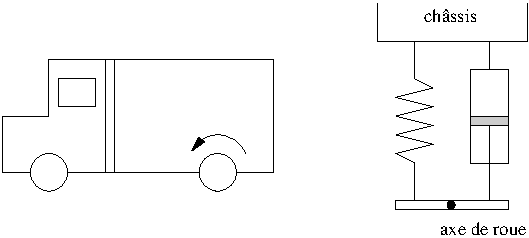
\includegraphics[width=3in]{exe-camion}
\caption{Modélisation de la dynamique d'un camion}
\label{Fig:exe-camion}
\end{center}
\end{figure}
Pour cela chaque voiture est munie d'un dispositif
actif qui applique une force verticale à la caisse de la voiture pour
contrebalancer l'effet de la force \og centrifuge \fg. Ceci est illustré sur
la figure \ref{Fig:train} où une section de la caisse d'une voiture est
représentée schématiquement avec $F_g$ la force de gravité
(appliquée au centre de masse $G$), $F_c$ la force "centrifuge" et
$F_a$ la force appliquée. On suppose que la ligne d'action de la force
$F_a$ est verticale quelle que soit la position angulaire $\theta$ de la
caisse. D'autre part la suspension de la voiture est schématisée par
un ressort vertical qui exerce une force proportionnelle à son
élongation. Le point d'application
$P$ du ressort est {\it contraint de se déplacer verticalement}.
Etablir un modèle d'état du système. \qed
\end{exercice}
\vv

\begin{exercice}{\bf \em Modélisation de la dynamique d'un camion}

On considère un camion se dépla\c cant en ligne droite (Fig. \ref{Fig:exe-camion}), sous les hypothèses de modélisation suivantes~:
\begin{itemize}
\item[a)] Le camion est un système articulé composé de corps rigides (caisse et
roues).
\item[b)] Le camion est équipé d'une propulsion arrière (le couple développé par
le moteur est transmis aux roues arrières).
\item[c)] Les roues roulent sans glisser.
\item[d)] Les roues sont reliées au chassis par un système de suspension composé
d'un ressort linéaire et d'un amortisseur à frottement visqueux de masse
négligeable.  Ce système de suspension ne permet que des déplacements verticaux.
\end{itemize}
\begin{enumerate}
\item Etablir un modèle d'état du système qui satisfait ces hypothèses de
modélisation (se limiter à deux corps : le chassis et une roue motrice).
\item Quelles sont les principales limites de validité de ce modèle ? \qed
\end{enumerate}
\end{exercice}
\vv

\begin{exercice}{\bf \em Un bateau}

Un bateau muni d'un moteur orientable de type \og hors-bord \gf se déplace sur un fleuve comme illustré à la figure \ref{bateau} (vue du dessus). Le fleuve est de largeur constante (= 2$L$). La poussée du moteur est représentée par le vecteur de longueur $F$ (= grandeur de la force de propulsion) et d'orientation $\beta$. Le bateau est aussi soumis à la force du courant du fleuve qui est une fonction parabolique de l'abscisse $y$ : le courant est nul aux deux bords et maximum au milieu du fleuve. Quand le moteur est à l'arrêt, le bateau est entraîné à la vitesse du courant par la force de frottement de l'eau sur la coque. 
\begin{enumerate}
\item Etablir un modèle d'état du système. Pour simplifier, on peut supposer que :
\begin{itemize}
\item[a)] le bateau est un corps rigide de masse constante;
\item[b)] le plan d'eau est quasi-horizontal et la gravité n'influence pas le mouvement du bateau;
\item[c)] la force exercée par le courant s'applique ponctuellement au centre de masse du bateau (on néglige le fait que la force du courant peut s'exercer de manière variable en divers points de la coque).
\end{itemize}
\item Quelle doit être la capacité de propulsion du moteur pour que l'on ait la garantie que le bateau pourra remonter le courant ? \qed
\end{enumerate} 
\begin{figure}[h]
\begin{center}
\includegraphics[width=10cm]{bateau}
\caption{Un bateau}
\label{bateau}
\end{center}
\end{figure}
\end{exercice}
\vv



\end{document}
